%!TEX root =  mainMastersProject.tex

\chapter[State of the Art]{State of the Art}

\section{The problem with evidence}

When we find evidence for a hypothesis that we have held in the back of our minds, we then find the hypothesis more likely. 
This is the basic idea behind reasoning with evidence. In a constellation of hypotheses and pieces of evidence, we want
to construct a network that will lead us to believe as many true hypotheses as possible, given the evidence that we have.

However, evidence itself is elusive, and it's connection to hypotheses is as well - how can we be sure that some evidence supports
some hypothesis, and even if we know that it does, how can we express how strong the piece of evidence is? Some evidence
is very weak, and only after a tedious process of ruling out other factors and careful investigation and collection of other pieces
of evidence, we can come to a conclusion about a hypothesis. On the other hand, some evidence is so strong that it leaves no room for doubt.

We all have intuitions about evidence strength - but can we make these intuitions precise? Additionally, can we manage the complex
realities of weak evidence for many different hypothesis? These are questions that have guided this state of the art section.

In this section I will briefly discuss methods for reasoning with evidence, then transition to probabilistic reasoning with evidence,
Bayesian Networks. I will discuss some problems with Bayesian Networks.

\section{Reasoning with evidence}
Argumentation graphs and their semantics.
Scenario theory.
Bayes Law.
Hybrid Approach.

\section{Bayes!}
Probabilistic reasoning (Dahlman, simple).
Bayesian Networks
Vlek and Timmer
Fenton and Vlek - combining scenarios, idioms in Bayesian Networks.

\subsection{Bayesian Networks}
DAG. Pearl. Random variables nodes, ``causal'' but actually conditional.


Advantages:

Disadvantages: The use of Bayesian Networks is not straightforward, neither for the builder or for the interpreter (de Koeijer): it is complex, time-consuming, hard to explain, and, the `repeatability [...] leaves much to be desired. Node definitions and model structures are often directed by personal habits, resulting in different models for the same problem, depending on the expert' (de Koeijer).


\subsection{(Automatic) Bayesian Networks Builders}
Standard toolsets. Pyagrum, agenarisk and hugin. We build Bayesian Networks by hand, perhaps guided by a scenario or by argumentation. However, the links that we put between nodes must be done by ourselves.

The standard way of building Bayesian Networks in law, is for now, based on human intuition. Usually, in other domains, we can build Bayesian Networks automatically from large datasets using algorithms such as K2. Automated Bayesian Network building is not plausible in the legal-evidence domain, because the data that we need is notoriously sparse - we have information about the number of crimes, from police departments, but for the subaspects for each scenario, it is hard to find frequencies (reference class problem, and others).

However, since we're using simulations to investigate the Bayesian Approach, we can generate a near infinite amount of information, and then we use this information to build the network, such as we might use data on health markers to predict kidney failure (medical domain - pretty sure this is the standard example). So automated building tools come in handy. In this project I only used the K2 algorithm, because you can add temporal information to it.

{\color{red}Explain K2 algorithm here.}

Automated Bayesian Network building might prove useful in other, more data-and-information-rich legal subdomains - such as pure forensics (DNA evidence), or case-outcome prediction.


\section{Problems with the Bayesian Approach}
There are many problems with the Bayesian Approach.

The most obvious is the problem of the numbers: where do we get them? We can get some of them from statistics, but we need to many numbers that we have to make some numbers up. This is not necessarily a bad thing - we put our (betting) money where our mouth is and assign numerical precise probabilities to situations that we preciously only had vague intuitions for. However, this brings about the veil of objectivity. By giving a probability to your intuitions, you have made your intuitions more precise and you can now reason with them, update on evidence using Bayes Law, and everything's great. In some domains, this is obviously okay. If you want to bet cents on world events and walk that fine line between calibration and discrimination for fun and profit, that's no problem.  After all, there are incentives to abstain from the unclear, the stuff that might not have a specified answer, the vague. But when we are talking about using evidence in law, we are talking about exactly that domain - we're not making predictions about the price of oil in 6 months, or the outcome of the French election, with clear outcomes, clear procedures for measurement. Instead, we're trying to make predictions about crimes and crime scenarios, which are a lot vaguer, and strangely unobservable at times - things like motives, or behaviours that happen under specific circumstances, interlocking stuff with complex dependencies. We all have intuitions about evidence strengths in vague situations, but they are more difficult to make precise than the traditional `forecasting' events. So trying to assign probabilities without a clear method of calibration, makes that they will be imprecise.

Level of granularity.

Independence relations. Selecting events.

Technical problems with Bayesian Networks. Precision. Evaluation. Sensitivity Analysis.

\begin{enumerate}
\item The problem of the reference class, which is also a problem within a `clear' domain - but this is a fundamental philosophical problem that I will not discuss further.
\item We do not know the probabilities (frequency) of our variables in the first place.
\item We do not know how robust the network is to imprecise or wrong frequencies.
\item We do not know if the assumption of independence between any two variables holds. The assumption of independence is necessary in Bayesian Networks, otherwise the complexity of the network becomes unmanageable.
\end{enumerate}


\section{Background on probabilities - the meaning of random variables}

Bayesian Networks consists of nodes, and arcs between those nodes. The nodes in a Bayesian Network are random variables. But what are random variables? 

Well, a random variable (RV) is not just a natural language statement, but it's a mathematical object. It is a function or mapping of the form $X : \Omega \rightarrow S$, where $\Omega$ is the universe, and $S$ is the sample space. The RV maps some elementary event in the universe, to a specific output in sample space (Figure~).


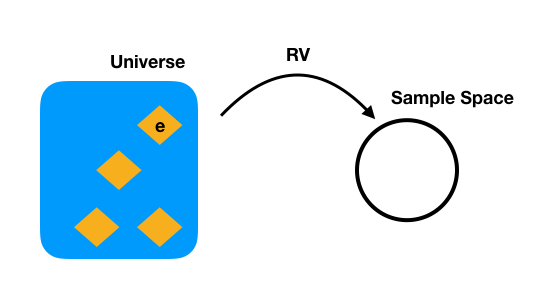
\includegraphics[width=\linewidth]{images/rv1.png}


This is not really an explanation, because 1) what is a universe? 4) what is a sample space? 3) mapping how? 2) what is an elementary event? and so on.

The universe can be super abstract. It is the place where the events happen that we're interested in. It can be our actual universe, a simulation, or a subset or our actual universe or simulation. Elementary events are the events that happen within our universe - they are the elements of the set that is the universe. A random variable is a procedure, with a method, that can map an event to a certain value. All the possible values that an event can take, are collected in the sample space S. \footnote{This is how far I'll go with this explanation, if you want to know about $\sigma$-fields I don't have time to understand and explain all of that. And I don't think its necessary for the problems with bayesian networks.}

To illustrate this, we have a simple example (Example~1).


\begin{example}
Let's say that we are observing a painter who wants to put down the first layer of paint on their canvas. The painter has to pick the color of the background layer. $\Omega$ is the universe, and contains all events where this painter is picking a color for a background for an oil painting. $\S$ is the sample space, and is the set of all colors that the painter can pick. The RV $X$ maps events to values in sample space. For this initial simple example, $S = \{green, blue, orange\}$. Then $X^{-1}(orange)$ refers to the set of all events where the painter picked "orange" as the background color.

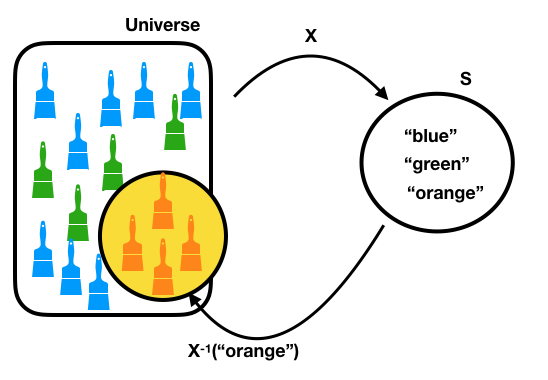
\includegraphics[width=\linewidth]{images/rv2.png}
\end{example}

In our example, we say that the RV $X$ maps events to values in sample space (and inversely, $X^{-1}$ maps a value in sample space to a set of events). However, how does this mapping work? The mapping itself is not a mathematical object (eg, we don't do $X(\omega) = 2*\omega^2 = "orange"$). Instead, we observe a certain event $w$ in $\Omega$, and measure in some way, to find out what value $w$ takes in $S$. For things like dice-rolls, it is clear how we observe the event (we just look at it), just like in our painting example. However, there are several ways that we can observe and map this situation, operationalise it, which all respond to different RV's:

\begin{enumerate}
\item \textbf{RGB Color-picker}: we take a picture of the canvas, and analyse it in the computer. We have selected certain ranges of RGB values that correspond to orange, blue and green, respectively. The average color of the canvas within one of the RGB-color bins is how we know what color it is.
\item \textbf{Taste}: we have a super-taster who specialises in paint pigments \footnote{Not the healthiest of occupations.}. When she blind-tastes a bit of the paint, she can tell us what color it is, because the pigment that causes the color orange tastes different from the green, which tastes different from blue.
\item \textbf{Subjective taste}: I have my own opinions on whether some paint color is orange, blue or green. I see the canvas, and I decide \footnote{I might be colorblind}.
\item Think of something else ridiculous.
\end{enumerate}

Of these operationalisations of the RV you can think many things. Some might be more valid than others. We can only know if we trust the final probability assignment (I will get there in a second) if we can agree with the method of mapping - which is the random variable. The operationalisation of the random variable is a big deal, and to know if it is valid/accurate, we need to know exactly how it was mapped, because then we can argue about it if we don't like it.

Now, let's assume we have some sort of way of determining the color of the canvas (really does not matter which one, as long as we pick one). Then, we can talk about probability! Probability maps an event to a real number $[0, 1]$. The `event' here is not the same as an elementary event. Instead, `event' means that a RV takes some value in the sample space - so an event is the set of elementary events in the universe, for which the random variable on that event takes a specific value - $\{\omega \in \Omega \vert X(\omega) \in orange\}$ is the set of cases where the color on the canvas is orange.

Then, we can assign a probability value to this event, simply $P(X \in A) = p$. There's a whole debate on what $p$ should actually mean - is it a degree of belief, or a frequency, or something else? The frequentist view is that we repeat measurements - eg, we apply the RV a lot (every time the painter is starting a new painting), and count how often the canvas is orange, and then divide that by the total amount of new canvases started, and this should be the value of $p$.  In the subjectivist view, $p$ can be any value as long as that value reflects our belief on how many times the painter paints orange vs blue vs green backgrounds. Then, we have our probability! 

A different problem is for our universe. Are we only counting oil paintings, or are we also counting acrylics. Or did we say `painting' when we meant `artwork' and should we also take the painter's sketches and pastel drawings into account? This is the second problem, and it is known as the problem of the reference class. Different reference classes will result in different frequencies (also in different degrees of belief). That's why it is not just important to specify operationalisations for every random variable, but also specify exactly what part of the universe you're investigating (eg, what is and isn't in $\Omega$).


\section{Agent simulations}
Why are simulations a good tool for investigating problematic aspects of the application of Bayesian Networks in law? Primarily, simulations are useful because they are a completely determined environment. This means that we can know exactly with what frequencies events occur, generating lots of data for our K2 algorithm to build networks with.

But are agent simulations even used in crime? Is this purely an academic exercise? Actually yes, but maybe also no.
Bosse and Gerritsen and friends.

\section{What's the point? Conclusion and Normativity}

In this chapter I have laid out the landscape of theories that I'm going to travel in the rest of this thesis. The two main ideas are Bayesian reasoning, specifically as implemented in Bayesian Networks, and computational simulations of agents. The simulation is supposed to be the grounding for the Bayesian Networks.

But why do we want to use Bayesian Networks in the first place? In the best possible case, a Bayesian Network would help us to make the correct reasoning steps, telling us exactly how to weigh each piece of evidence in the grand scale of the simulated crime. This is a normative approach - it's telling us how to reason, but it is not (and not meant to be) an empirical approach. As far as I know, Bayesian networks are not a reflection of `how people actually reason' - eg if you open up our minds, you won't see Bayesian Networks in there. One of the problems for normative models in decision making (see Colyvan 2013), is that we can only test how well our normative models work, if we already know what a good outcome would be. In a sense, we're doing experimental model testing for normative Bayesian Networks in this project.

 



